\chapter{Построение решения}
\label{cha:ch_3}
По большей части эта работа повторяет метод из \cite{Bonjean}, однако кроме упомянутых каталогов 
PSZ2 и MCXC для сопоставления результатов использовался каталог ACT. Кроме того, детекция скоплений 
производилась следующим образом:\\

\begin{enumerate}
    \item Для сканирования выбирается один пиксель из разбиения HEALPix с $n_{side} = 2$\\
    \item Чтобы просканировать всю область, нужно пройтись по ней окном $64 \times 64$. Для этого 
        нужно выбрать шаг сканирования - можно задать его как $64$, тогда сканирование получится 
        без пересечений, однако при меньшем шаге результаты оказываются лучше\\
    \item Каждое изображение отправляется на вход в нейросеть. Полученные маски склеиваются и 
        усредняются, чтобы снова получить изображение размером с пиксель $n_{side} = 2$\\
    \item На полученной маске отделяются области со значениями, превышающими заданный порог\\
    \item Для каждой области определяется её барицентр, который преобразуется в небесные координаты\\
\end{enumerate}

У полученных после детекции каталогов определяются следующие параметры для каждого из 
детектированных объектов:\\
\begin{itemize}
    \item area – площадь сегментированной области скопления\\
    \item min\_rad, max\_rad, mean\_rad – минимальный, максимальный, средний радиусы области\\
    \item min\_pred, max\_pred – минимальное, максимальное значение маски в области\\
    \item status – факт сопоставления скопления с объектом из каталога\\
    \item catalog --- сопоставленный каталог\\ 
\end{itemize}

\begin{figure}
    \center{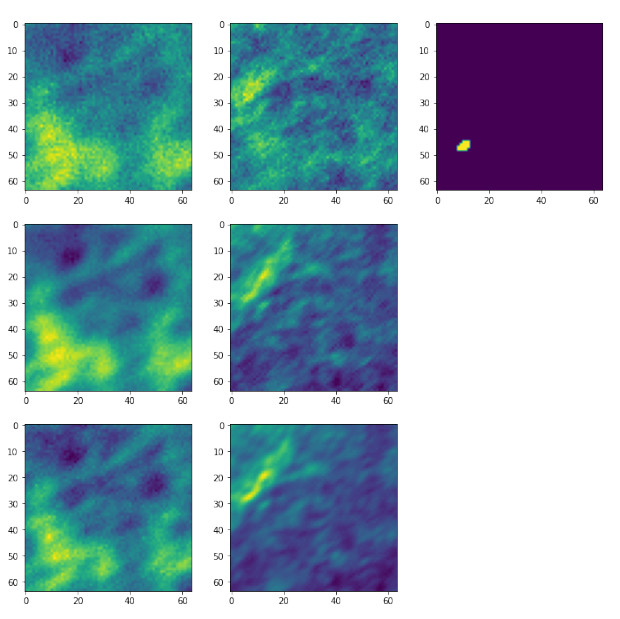
\includegraphics[width=0.5\linewidth]{patch}}
    \caption{Пример патча с шестью каналами данных Planck и маской с отмеченным центром скопления}
\end{figure}

На данный момент для детекции был выбран шаг сканирования $8$, так как это наименьший шаг 
сканирования, при использовании которого тратится вменяемое количество времени, кроме того, из всех 
возможных вариантов этого параметра это значение дает наилучшие результаты recall и fp на тестовой 
области:\\
\begin{figure}
    \center{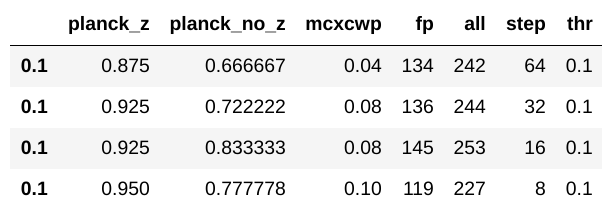
\includegraphics[width=0.6\linewidth]{step_comp}}
    \caption{Сравнение различных вариантов параметра шага сканирования}
\end{figure}

Однако предполагается, что при значения шага меньше $8$ результаты могут быть еще лучшие, но этот 
вопрос еще предстоит исследовать.\\

